\part[Ablauf, Organisation und Umfeld]{Ablauf, Organisation und Umfeld
    }

\tableofcontents

\chapter{Aufgabenstellung}

\section{Titel der Arbeit}
Hitobito: Neue Generation von Personen-Filtern

\section{Thematik}
Eines der Kernfunktionalitäten von Hitobito ist das Filtern via vom Benutzer definierten Kriterien von Personen auf Personenlisten und Abos. Diese Funktionalität ist in den über 10 Jahren seit es Hitobito gibt oft erweitert worden. Durch die vielen neuen Filtermöglichkeiten wurde speziell das UI immer komplexer und unübersichtlicher. Die Personen-Filteroptionen für Personenlisten und die der Abos sehen ähnlich aus, weisen aber diverse nicht offensichtliche Unterschiede auf. Mit dieser Probe-IPA soll für den Backendteil der Abos (MailingLists) eine neue Generation von Personen-Filtern für Hitobito entwickelt werden.

\section{Ausgangslage}
Hitobito ist eine Open Source Webapplikation zum Verwalten von Mitgliedern, Events und vielem mehr. Die Ruby on Rails Applikation wurde 2012 von Puzzle ITC initiiert und wird stets weiterentwickelt.

Die Basis für die Software bildet das Webframework Ruby on Rails. Für das User Interface wird neben statischer Technologie wie HTML und CSS auch JavaScript oder Hotwire verwendet. Der komplette Source-Code steht auf Github zur Verfügung: https://github.com/hitobito

\section{Detaillierte Aufgabenstellung}
Mit dieser Probe-IPA soll ein neues Konzept und Datenmodell für die Persistierung von Filter-Parametern erstellt werden (rein Backend). Anschliessend soll dieses Konzept in einem Proof of Concept (PoC) bei einem Teil der Mailinglisten (Abos) umgesetzt werden.

\begin{itemize}
    \item Die Klassen Subscription, RelatedRoleType, PeopleFilter, usw. werden im neuen Konzept komplett ersetzt oder ggf. ergänzt
    \item Eine Möglichkeit ist das PeopleFilter die Basis für das neue Konzept bilden
    \item Es sollen 2-3 Grobkonzepte gegenüber gestellt werden und das ausgewählte Konzept detaillierter ausgearbeitet werden
\end{itemize}

PoC

\begin{itemize}
\item Folgende Komponenten der MailingLists Filter sollen mit dem neuen Konzept im PoC umgesetzt werden:
    \begin{itemize}
        \item Globale Bedingungen > Sprache
        \item Personen
        \item Ausgeschlossene Personen
        \item Optional: Gruppen / Rollen
    \end{itemize}    
\item Persistierte Subscriptions/Filter müssen für den PoC vorerst nicht migriert werden
\item Die nicht erwähnten Komponenten müssen nicht mehr funktionieren
\item Die erwähnten Komponenten (ohne Optionale) funktionieren im UI und haben eine minimale, funktionierende Testabdeckung (happy path)
\end{itemize}

\newpage

Out of Scope - wird nicht oder erst nach der Probe IPA umgesetzt

\begin{itemize}
    \item Konzept und Anpassungen Frontend/UI
    \item PoC Umbau/Migration People Filter Personenlisten
    \item JSON API Filter (Grafiti)
\end{itemize}

\newpage

\subsection{Mittel und Methoden}

Technologie und Plattform:

\begin{itemize}
    \item Ruby, Ruby on Rails, Active Record
\end{itemize}

Entwicklungsumgebung:

\begin{itemize}
    \item Intellij
    \item Git, Github
    \item Rake
    \item Rubocop
\end{itemize}

Textverarbeitung und Diagramme:

\begin{itemize}
    \item Latex
    \item draw.io
    \item Google Sheets
\end{itemize}

Projektmethode:

\begin{itemize}
    \item Scrum IPA
\end{itemize}

Konventionen:

\begin{itemize}
    \item Es gilt der \href{https://github.com/rubocop-hq/ruby-style-guide}{Ruby Style Guide} und der \href{https://github.com/rubocop-hq/rails-style-guide}{Rails Style Guide} gemäss Rubocop \href{https://github.com/puzzle/cryptopus/blob/master/.rubocop.yml}{Konfiguration des Projekts}
\end{itemize}

\subsection{Vorkenntnisse}
Marc arbeitet bereits seit einigen Monaten an Features von Hitobito. Ausserdem hat er bereits seit dem 2. Lehrjahr Erfahrung auch in anderen Ruby on Rails Projekten gesammelt.

\subsection{Vorarbeiten}
\begin{itemize}
    \item Vorbereitung Dokumentvorlage
    \item Ist-Analyse Personen-Filter Personen-Listen/Abos
    \item Dokumentation in der Developer-Dokumentation der bestehenden Implementation von MailingLists, FilteredList, Personen-Filter
\end{itemize}

\subsection{Neue Lerninhalte}

\begin{itemize}
    \item Eigenständiges Entwerfen der Datenstruktur/Klassen
\end{itemize}

\subsection{Arbeiten in den letzten 6 Monaten}

\begin{itemize}
    \item Umsetzung diverser Features für Hitobito (Ruby on Rails)
    \item Postgresql Migration Hitobito
\end{itemize}

\chapter{Firmenstandards}

\section{Code conventions}
Als Code convention werden die Ruby \href{https://github.com/rubocop/ruby-style-guide}{Style Guides} verwendet. 
Die Überprüfung dieser Style Guidelines wird mit Rubocop (Formatter) sichergestellt. Die Konfiguration
dieses Formatters ist unter \href{https://github.com/hitobito/hitobito/blob/master/.rubocop.yml}{rubocop.yml} ersichtlich.

\subsection{Lizenz}
In jedem File in Hitobito wird das Copyright für den jeweiligen Kunden und die Lizenz dazu
in Kommentarform beschrieben. Diese Lizenz- sowie Kundeninformationen können über folgenden Befehl 
eingefügt werden.

\begin{verbatim}
    rake license:insert
\end{verbatim}
    
Alternativ dazu können diese Informationen mit 

\begin{verbatim}
    rake license:remove 
\end{verbatim}

entfernt oder mit 

\begin{verbatim}
    rake license:update 
\end{verbatim} aktualisiert werden.

\newpage

\section{Git conventions}
Für das cloudbasierte Hosting unseres Git-Repositories wird Github verwendet. 
Die Git Commitnachrichten werden nach den Regeln von Puzzle ITC formuliert. Im Anhang
unter \hyperref[sec:gitconv]{Git Conventions} finden sie eine Kopie unserer Firmenkonventionen

\begin{itemize}
    \item Sprache: Englisch
    \item Kurze und prägnante Message, idealerweise unter 50 Zeichen \href{https://cbea.ms/git-commit/#limit-50}{Details}
    \item Mit Grossbuchstaben beginnen \href{https://cbea.ms/git-commit/#capitalize}{Details}
    \item Kein Punkt am Schluss \href{https://cbea.ms/git-commit/#end}{Details}
    \item Den \textit{imperative mood} (Befehlsform) verwenden, also «Fix bug with X» statt «Fixed bug with X» oder «More fixes for broken stuff» \href{https://cbea.ms/git-commit/#imperative}{Details}
    \item Wenn vorhanden Ticket referenzieren:
    \begin{itemize}
        \item Bei Open Project Work Packages: «Add X, refs \#12345»
        \item Bei Gitlab/Github Issues: «Add X \#12345»
    \end{itemize}
\end{itemize}

\section{Documentation Conventions}
Als Documentation covention wird arc42 verwendet (Siehe \href{https://arc42.org/documentation/}{arc 42 documentation}). 

\chapter{IPA-Schutzbedarfanalyse}

\section{Datensicherheit}
Die notwendigen Daten welche im Rahmen der IPA zu Test- und Vorführungszwecken verwendet werden,
sind werden durch das \href{https://github.com/faker-ruby/faker}{Faker-Gem} generiert und sind somit NICHT 
besonders schützenswert. Dazu gehören unter anderem Adressen, Familiendaten, Finanzdaten.

\section{Applikationssicherheit}

Da keine besonders schützenswerte Daten verwendet werden, werden die Standards von
Puzzle ITC nach Firmen-Sicherheitsbuch verwendet. Sie können dieses unter \hyperref[sec:secconv]{Security Conventions}
einsehen. Diese Security Conventions umfassen:

\begin{itemize}
    \item{Injection / Cross Size Scripting}
    \begin{itemize}
        \item{Input Validierung von allen Inputs serverseitig durchführen}
        \item{Output Encoding auf allen Outputs anwenden}
        \item{Kein inline oder dynamisches SQL, sondern parametrisierte Queries verwenden}
        \item {Datei Uploads überprüfen}
    \end{itemize}
    \item Verbindungs- / Browsersicherheit
    \begin{itemize}
        \item{Nur HTTPS verwenden und korrekt konfigurieren}
        \item{Security Headers setzen}
        \item{Cookie Flags secure, httpOnly und SameSite setzen}
        \item{Kein Caching von sensiblen Informationen}
    \end{itemize}

    \newpage

    \item Authentication / Sessions
    \begin{itemize}
        \item{IAM des Frameworks oder besser Keycloak verwenden}
        \item{Keine sensitiven Infos in URL Parameter}
        \item{Brute Force Schutz}
        \item{ Sessions schützen}
    \end{itemize}
    \item Tools und Betriebsumgebung
    \begin{itemize}
        \item{Errorhandling und Logging}
        \item{Libraries und deren Dependencies auf bekannte Schwachstellen prüfen}
        \item{OS, Webserver, Container aktuell halten und Hardening}
        \item{Keine Produktionsdaten auf Integrationsumgebungen}
    \end{itemize}
    \item Security Testing
    \begin{itemize}
        \item{Es dürfen keine Secrets im Repository abgelegt werden}
        \item{Eingebundene Dependencies dürfen keine MEDIUM und HIGH Schwachstellen aufweisen}
        \item{Eine statische Codeanalyse sollte durchgeführt werden}
        \item{Eine dynamische Codeanalyse sollte durchgeführt werden}
        \item{Alle verwendeten Images sollten auf Schwachstellen gescannt werden}
    \end{itemize}
\end{itemize}

\chapter{Organisation der IPA-Ergebnisse}

\section{Datensicherung}
In dieser IPA unterteilen wir die Datensicherung in:

\begin{itemize}
\item Dokumentation
\item Code
\end{itemize}

\subsection{Dokumentation}
\begin{table}[h!]
      \begin{tabular}{|L{0.4\textwidth}|L{0.5\textwidth}|}
          \hline
          \rowcolor{puzzleblue} \multicolumn{2}{|l|}{\color{white}\textbf{Dokumentation}} \\[12pt]
          \hline
          Tools & Git und USB \\
          \hline
          Versioniert & Ja \\
          \hline
          Interval & Mind. 2x täglich \\
          \hline
          Beschreibung & Die Dokumentation ist im ipa-puzzle-template Repository unter dem Branch probe-ipa angelegt.
          Sobald ein Dokumentationsticket abgeschlossen wurde, werden die Änderungen auf den Github Server in das private Repository
          gepushed. Dies geschieht mind. 2x täglich. Zusätzlich, wird pro Tag ein Ordner auf einem USB-Stick erstellt.  Am Ende des Tages wird eine Kopie der Dokumentation
          in diesen Ordner geladen. \\
        \hline
        \end{tabular}
        \caption{Sicherung Dokumentation}
  \end{table}

\newpage

\subsection{Code}
\begin{table}[h!]
    \begin{tabular}{|L{0.4\textwidth}|L{0.5\textwidth}|}
        \hline
        \rowcolor{puzzleblue} \multicolumn{2}{|l|}{\color{white}\textbf{Code}} \\[12pt]
        \hline
        Tools & Git und USB \\
        \hline
        Versioniert & Ja \\
        \hline
        Interval & Mind. 2x täglich \\
        \hline
        Beschreibung & Für die Entwicklung habe wurden die Repositories hitobito und hitobito\-generic geforked.
        Auf diesen Repositories wird an Tagen an welchen Entwickelt wird, mind. 2x täglich committed. An diesen Tagen
        wird zur doppelten Sicherung zusätzlich eine Kopie des Projektes auf den USB Stick gespeichert, unter dem Ordner des jeweiligen Tages. \\
      \hline
      \end{tabular}
      \caption{Sicherung Code}
\end{table}

\subsection{Wiederherstellung des Codes}
Gehen die Daten lokal verloren, können diese entweder über das Github Repository oder den USB-Stich wiederhergestellt werden.
Bei der Wiederherstellung mit Git, wird der SSH-Key des Repositories benötigt, damit dieses von Github geklont werden kann. Ist
dieser SSH-Key nicht verfügbar, wird die Wiederherstellung über den USB-Stick vorgenommen und das Projekte des letzten Speicherstandes
kopiert. Im Falle des USB-Sticks sind mit mehr Datenverlusten zu rechnen, falls der Datenverlust gegen Mittag oder Nachmittag auftritt, da
die Speicherung erst am Ende des Tages erfolgt. Aus diesem Grund ist die Datenwiederherstellung mit Git zu bevorzugen.

Die Nachweise für die jeweiligen Datensicherungen finden sie im Anhang unter: TODO(Screenshots in Anhang einfügen)
\begin{itemize}
    \item \hyperref[sec:savusb]{USB-Sicherung}
    \item \hyperref[sec:savgit]{Git-Sicherung}
\end{itemize}

\chapter{Projektmethode}
Die verwendete Projektmethode dieser IPA ist SCRUM. Abweichungen und Werkzeuge welcher der Umsetzung
dieser IPA nach SCRUM verwendet werden, sind im folgenden Abschnitt beschrieben.

\section{Github Board}
Um die Userstories, Aufwandschätzungen und den Projektstatus zu verfolgen verwende ich Github Projects. 

\subsection{Backlog}
Zu Beginn der IPA wurde ein Backlog erstellt indem alle User Stories aufgeführt werden. Die Stories im Backlog
müssen noch nicht detailliert spezifiziert sein, sie dienen dazu eine Übersicht über noch offene Aufgaben während
der IPA zu erhalten.

\subsection{Refinement}
In der Refinement Spalte werden die Userstories vor dem Sprint Planning detaillierter beschrieben und mit Akzeptanzkriterien versehen. 
Der Detailbeschrieb dient dazu die Story später im Sprint Planning besser schätzen zu können.
Falls eine Userstory zu gross wird, wird sie in dieser Spalte auf zwei oder mehrere Stories unterteilt. Ausserdem werden pro Userstory Akzeptanzkriterien
definiert welche erfüllt werden müssen um diese während des Sprints abzuschliessen.

\newpage

\subsection{Sprint Backlog}
Anfangs Sprint wird immer ein Sprint Planning durchgeführt. Dabei werden die Userstories geschätzt und in den Sprint Backlog gezogen. 
Am Ende des Sprints sollte der Sprint Backlog leer sein. Ist dies nicht der Fall muss die Story zurück ins Refinement, neu beschrieben werden 
(falls Änderungen aufgetaucht sind) und muss dann in den nächsten Sprint weitergezogen werden.

\subsection{In Progress}
Während des Sprints werden Ticket in die In Progress-Spalte geschoben sobald die Arbeit daran beginnt.

\subsection{Done}
Eine Userstory kann in die Done-Spalte gezogen werden, wenn alle Akzeptanzkriterien erfüllt wurden.
Die Story gilt danach als abgeschlossen.

\section{Sprints}
Die gesamte IPA wird in drei Sprints unterteilt, diese umfassen je eine der folgenden
Phasen:

\begin{itemize}
\item Initialisierung
\item Umsetzung
\item Finalisierung    
\end{itemize}

Jedes Ticket wurde mit einem der Phasen gelabeled. So kann abgeschätzt werden, welche Tickets in welchem
Sprint erledigt werden müssen.

\section{Sprint Planning}
Das Planning findet immer zu Beginn des nächsten Sprints statt. Während des Sprint Plannings werden die zu erledigenden
Stories vom Refinement in den Sprint Backlog geschoben und geschätzt. Um die Planung im Zeitplan
besser darzustellen, wird definiert dass die Stories in Stunden anstatt Story Points geschätzt werden. Die niedrigste Schätzung
entspricht dabei einem Betrag von 0.5 Stunden.

\section{Daily}
Jeden Morgen findet ein Daily mit der verantwortlichen Fachkraft und der zusätzlichen verantwortlichen Fachkraft statt
welche den Stand des Sprintes prüfen und offene Fragen von mir beantworten. Ausserdem präsentiere ich im Daily den Stand der 
Dokumentation welche meine zuständigen Fachkräfte prüfen und mir Tipps zur Verbesserung geben. 

\section{Verwendungsgrund}
Die Projektvorgehensmethod wurde so gewählt, da sie für die IPA mehrere Vorteile bringt:

\begin{itemize}
    \item \textbf{Sprint Ende:} SCRUM zwingt den Entwickler dazu am Ende des Sprintes ein brauchbares Produkt zu haben
    \item \textbf{Agilität:} Wenn eine Story nicht erreicht wurde, kann sie in den nächsten Sprint gezogen werden
    \item \textbf{Daily:} Durch die Dailies wird ein täglicher Austausch zwischen Fachkraft und Kandidat sichergestellt
    \item \textbf{Akzeptanzkriterien:} Mit den Kriterien verhindern wir das abschliessen von halbfertigen Features oder fehlerhafter Software
    \item \textbf{Board:} Durch das Github Projects Board ermöglichen wir eine schnelle Übersicht über den Stand der IPA

\end{itemize}

\chapter{Projektaufbauorganisation}
\section{Projektrollen in Scrum}
\begin{figure}[h]
    \centering
    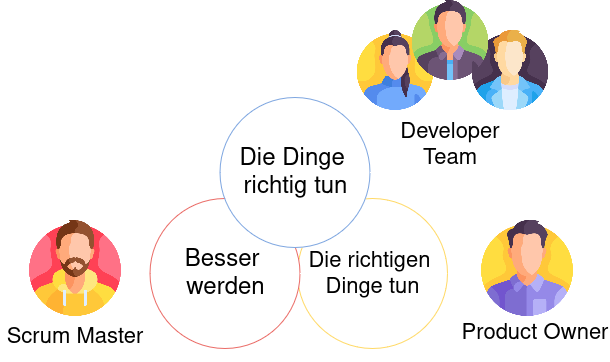
\includegraphics[width=1\textwidth,]{scrum_roles.drawio.png}
    \caption{Rollen in Scrum}
\end{figure}


\begin{table}[h!]
        \begin{tabular}{|L{0.4\textwidth}|L{0.5\textwidth}|}
            \hline
            \rowcolor{puzzleblue} \multicolumn{2}{|l|}{\color{white}\textbf{Rollenbeschreibung}} \\[12pt]
            \hline
            Product Owner & Der Product Owner vertritt die Interessen des Kunden. Er priorisiert die Aufgaben im Product Backlog  \\
            \hline
            Scrum Master & Der Scrum Master coached die Entwickler und beseitigt Hindernisse. Er sorgt für eine 
            kontinuierliche Verbesserung in der Arbeit. \\
            \hline
            Entwicklerteam & Das Entwicklerteam arbeitet selbstorganisiert den Sprint Backlog ab. 
            Durch Dailies wird ein laufender Informationsaustausch sichergestellt. \\
            \hline
          \end{tabular}
          \caption{Rollenbeschreibung}
\end{table}

\section{Projektrollen IPA}
\begin{table}[h!]
    \begin{tabular}{|L{0.4\textwidth}|L{0.5\textwidth}|}
        \hline
        \rowcolor{puzzleblue} \multicolumn{2}{|l|}{\color{white}\textbf{Rollenbeschreibung}} \\[12pt]
        \hline
        Verantwortliche Fachkraft & Unterstützt den Kandidaten von seiten des Lehrbetriebes. Erste Anlaufstelle bei Problemen.  \\
        \hline
        Zusätzliche verantwortliche Fachkraft & Unterstützung für die verantwortliche Fachkraft \\
        \hline
        Experten & \textbf{Validierungsexperte:} Validiert die IPA-Aufgabenstellung.
                    \textbf{Hauptexperte:} Verantwortlich für die Bewertung der IPA.
                    \textbf{Nebenexperte:} Unterstützung für den Hauptexperten. \\ 
        \hline
      \end{tabular}
      \caption{Rollenbeschreibung}
\end{table}

\newpage

\section{Rollenverteilung}
\begin{figure}[h]
    \centering
    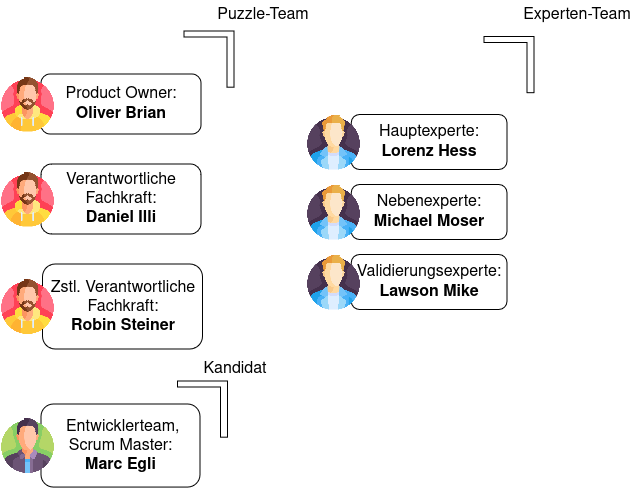
\includegraphics[width=1\textwidth,]{rollenverteilung_ipa.drawio.png}
    \caption{Rollen in Scrum}
\end{figure}

\begin{table}[h!]
    \begin{tabular}{|L{0.4\textwidth}|L{0.5\textwidth}|}
        \hline
        \rowcolor{puzzleblue} \multicolumn{2}{|l|}{\color{white}\textbf{Rollenbeschreibung IPA}} \\[12pt]
        \hline
        Verantwortliche Fachkraft & Daniel Illi  \\
        \hline
        Zusätzliche verantwortliche Fachkraft & Robin Steiner \\
        \hline
        Validierungsexperte & Lawson Mike \\ 
        \hline
        Hauptexperte & Lorenz Hess \\ 
        \hline
        Nebenexperte & Michael Moser \\ 
        \hline
        Scrum Master & Marc Egli \\ 
        \hline
        Development Team & Marc Egli \\ 
        \hline
        Kandidat & Marc Egli \\ 
        \hline
      \end{tabular}
      \caption{Rollenbeschreibung IPA}
\end{table}


\chapter{Zeitplan}

\section{Erläuterung zum Zeitplan}
% TODO: Beschreibe den Zeitplan, um eventuelle Unklarheiten zu vermeiden

\newpage
\storeareas\zeitplan
\KOMAoptions{paper=a3, paper=landscape, DIV=current}
\areaset
  {\dimexpr\the\paperwidth-1cm\relax}% calculate requiered \textwidth
  {\dimexpr\the\paperheight-5.5cm\relax}% calculate requiered \textheight
\recalctypearea

% \begin{figure}[htp] \centering{
%     \includegraphics[scale=1]{zeitplan.pdf}}
%     \caption{Zeitplan IPA}
% \end{figure}

\restoregeometry
\zeitplan
\newpage



\chapter{Arbeitsjournale}
\section{Tag 1: 14.01.2025}
\begin{table}[H]
    \begin{tabular}{|L{0.4\textwidth}|C{60pt}|C{60pt}|C{60pt}|}
        \hline
        \rowcolor{puzzleblue}\color{white}Tätigkeiten & \color{white}Beteiligte \color{white}Personen & \color{white}Aufwand Geplant (std) & \color{white}Aufwand Effektiv (std) \\
        \hline
        Planning & Marc Egli & 1 & 1 \\
        \hline
        Zeitplan & Marc Egli & 2 & 2 \\
        \hline
        Aufgabenstellung übernehmen & Marc Egli & 1 & 0.5 \\
        \hline
        Standards aus Github übernehmen & Marc Egli, Nils Rauch & 1 & 1.5 \\
        \hline
        IPA Schutzbedarfanalyse & Marc Egli, Nils Rauch, Olliver Brian, Olliver Dietschi, Thomas Ellenberg & 1 & 0.75 \\
        \hline
        Scrum Beschrieb & Marc Egli & 1 & 1.5 \\
        \hline
        Arbeitsjournal & Marc Egli & 0.25 & 0.5 \\
        \hline
        Backupkonzept & Marc Egli & 1 & 0.25 \\
        \hline
        \textbf{Total} &  & 8.25 & 8.25 \\
        \hline
    \end{tabular}
    \caption{Tätigkeiten Tag 1}
\end{table}

\subsection*{Tagesablauf}
Heute bin ich motiviert in die IPA gestartet. Als erstes habe ich am morgen nochmals die Spezifikationen für
die Dokumentation, durchgelesen und das Template für die IPA angepasst. Nachdem ich eine passende Struktur hatte, 
startete ich auch schon direkt mit dem ersten Sprint Planning dieser IPA. Dabei habe ich alle Tasks für den Sprint 1
im Backlog erfasst, diese dann im Refinement detaillierter Beschrieben und am Schluss in den Sprint Backlog geschoben.
Die ganze Planung habe ich mit Gihub Projects gemacht, leider kam ich da bezüglich Issues an die Grenzen denn leider kann mann 
diese nur definieren wenn die Issues einem Projekt, welches NICHT geforked ist, zugewiesen werden können. Dieses Problem werde
ich am Daily morgen mit meiner Fachkraft besprechen, evtl. weis er mehr dazu. 

Nach dem Planning begann ich mit dem Bereitstellen des Zeitplans. Ich übernahm das Tempalte welches ich ausgewählt hatte und
passte es auf meine drei Sprints in den kommenden zwei Wochen an. Zuerst dachte ich, dass ich den Zeitplan schneller fertigstellen könnte
jedoch hatte ich Probleme mit Google Sheets und das anlegen von gemergeden Spalten dauerte lange. Trotzdem ist die Planung aufgegangen und nach 2 Stunden
hatte ich einen geeigneten Zeitplan. 

Am Nachmittag Startete ich direkt mit dem Dokumentieren, angefangen bei den Standards unserer Firma. Es dauerete länger als gedacht,
alle Standards zu sammeln und in die Struktur der Dokumentation zu bringen, weswegen ich dort etwas Zeit verlor. Ein Teil davon konnte ich dann
bei der Schutzbedarfsanalyse wieder reinholen. Hier suchte ich den Kontakt mit anderen Mitarbeitern, um herauszufinden wo das Datenschutzkonzept für
Hitobito hinterlegt ist. Anscheinend wusste das Niemand aussert Oliver Brian, welcher mir dieses für die Ablage im Anhang zur Verfügung stellte.

Gegen den Ende des Tages habe ich die Projektmethode Scrum Beschrieben und dokumentiert wie ich mich während der IPA organisieren werde. 
Bezüglich der Aufteilung der Spalten der User Stories bin ich hier noch unsicher, ich werde dies sicher morgen am Daily auch mit
Daniel Illi abklären.

\subsection*{Hilfestellungen}
\begin{itemize}
    \item Oliver Brian: Nachfrage Datenschutzkonzept
    \item Nils Rauch: Nachfrage Sicherheitskonzept / Sicherheitsconventions Puzzle ITC
\end{itemize}

\subsection*{Reflexion}
Ich konnte heute schon einiges dokumentieren und habe nun eine Vorlage von der aus ich
einfach weiterarbeiten kann. Zusätzlich habe ich mit Github Project einen Ort an dem ich meinen
Fortschritt verwalte und mich selbst organisiere. Probleme gab es nur bei der Beschaffung des Datenschutzkonzeptes
und der Arbeit mit Google Sheets.

\subsubsection*{Was lief gut}
Grundsätzlich lief das Dokumentieren selbst sehr gut. Ich konnte alle restlichen Informationen
für die Standars oder die Projektmethode schnell Beschaffen und mich dann dem Dokumentieren widmen. 

\subsubsection*{Was lief weniger gut}
Weniger gut lief die Arbeit mit Google Sheets und die Arbeit mit der Latex Vorlage. Zum Teil hatte ich
recht lange bis ich herausfand wie ich eine Liste anlege oder ein Bild einfügen kann. Ausserdem habe ich mich im 
Zeitplan verschätzt und heute 9.25 anstatt 8.25 Stunden geschätzt, da ich im Google Sheets einen Fehler gemacht habe. Diesen konnte
ich aber schnell korrigieren, so dass ich heute auf geplante 8.25 Stunden komme, welche ich nun auch erreiche.

\subsubsection*{Meine Erkenntnisse von heute}
Mit erweitertem Latex know-how und dem Datenschutzkonzept in den Händen kann ich nun weiter dokumentieren.
Ich denke ich werde somit auch weniger Probleme mit Google Sheets und Latex haben, da ich heute schon viele
meiner Probleme lösen konnte.

\subsection*{Nächste Schritte}
Als nächstes werde ich morgen das Backupkonzept fertig machen und dann direkt zur Projektaufbauorganisation 
gehen. Nach Abschluss dieser Story kann ich den Sprint 1 Abschliessen und schon in den Sprint 2, der Konzeption / Umsetzung
starten.

\pagebreak

\section{Tag 2: 15.01.2024}
\begin{table}[H]
    \begin{tabular}{|L{0.4\textwidth}|C{60pt}|C{60pt}|C{60pt}|}
        \hline
        \rowcolor{puzzleblue}\color{white}Tätigkeiten & \color{white}Beteiligte \color{white}Personen & \color{white}Aufwand Geplant (std) & \color{white}Aufwand Effektiv (std) \\
        \hline
        Backup Konzept & Marc Egli & 0 & 0.5 \\
        \hline
        Projektaufbauorganisation & Marc Egli & 2 & 2.25 \\
        \hline
        Standards & Marc Egli & 0 & 0.25 \\
        \hline
        Datenschutzkonzept & Marc Egli & 0 & 0.5 \\
        \hline
        Planning & Marc Egli & 1 & 1 \\
        \hline
        Daily & Marc Egli, Daniel Illi & 0.25 & 0.5 \\
        \hline
        Arbeitsjournale & Marc Egli & 2 & 0.25 \\
        \hline
        \textbf{Total} & & 5.25 & 5.25 \\
        \hline
    \end{tabular}
    \caption{Tätigkeiten Tag 2}
\end{table}

\subsection*{Tagesablauf}
Heute konnte ich dank den Erkenntnissen von gestern schnell mit der Latex Dokumentation
vorankommen. Das Backup-Konzept konnte ich direkt abschliessen und habe dort sogar noch eine
Viertelstunde gespart. Diese brauchte ich wiederum für die Projektaufbauorganisation. Was hier länger gedauert hat,
war das erstellen der Diagramme. Ich wollte die Scrum Rollen und Rollenverteilung möglichst übersichtlich machen, was Zeit
kostete. Zuletzt waren die Arbeitsjournale geplant, hier habe ich einen Fehler in meiner Planung gemerkt. Ich habe angenommen, dass
ich die Arbeitsjournale noch anpassen müsste und wegen der fehlenden Latex-Erfahrung habe ich deswegen zwei Stunden eingeplant.

Allerdings hatten wir schon ein Template für das Arbeitsjournal im Projekt, deswegen hat sich diese Zeit auf 0 Stunden reduziert. Die
übrige Zeit habe ich dafür aufgewendet Nachbesserungen an der Dokumentation im Bereich Datenschutzkonzept und Standards zu machen. Zudem hat
das Daily auch länger gedauert, welches die nötige Zeit dann rausholen konnte. 

Zum Schluss des Tages habe ich den Sprintabschluss und das Planning für die Umsetzungsphase
gemacht. 

\newpage

\subsection*{Hilfestellungen}
\begin{itemize}
    \item Nils Rauch: Nachfrage Tool für Erstellung des Zeitplans
    \item Daniel Illi: Nachfrage Datenschutzkonzept
\end{itemize}

\subsection*{Reflexion}
Heute konnte ich sehr erfolgreich mit der Latex Dokumentation arbeiten. Auch das Planning
lief gut, ich denke ich habe nun eine saubere Planung für die Umsetzungsphase welche mir genug
Spielraum lässt. Der Fehler mit dem Zeitplan und Arbeitsjournal hat mir zwar Zeit in der Dokumentation gekostet,
allerdings ist es besser zu viel Zeit als zu wenig geschätzt zu haben. 

\subsubsection*{Was lief gut}
Die Arbeit mit Latex ging heute ohne Probleme voran und meine Effizienz war heute deutlich grösser 
als gestern.

\subsubsection*{Was lief weniger gut}
Der Fehler im Zeitplan mit den Arbeitsjournalen hat mich in der Planung durcheinandergebracht.
Ich habe die Zeiten nun korrekt im Zeitplan vermerkt, damit keine weiteren Probleme darunter entstehen.

\subsubsection*{Meine Erkenntnisse von heute}
Ich sollte vor der Eintragung in den Zeitplan prüfen, ob nicht schon Dokumente existieren welche mir
einen Teil der Arbeit abnehmen. Ist dies der Fall, wie bei meinen Arbeitsjournalen kann ich die Aufwandschätzung um 
ein Wesentliches reduzieren.

\newpage

\subsection*{Nächste Schritte}
Morgen werde ich mit der Umsetzung der IPA starten. Dabei werde ich zuerst die Einführung in das Hitobito
Projekt dokumentieren und dann direkt in die Konzeption für eine Filterlösung der Personenlisten und Abos starten.
Dies ist ein Schritt der mich zusätzlich motiviert, denn ich kann endlich etwas anderes machen als dokumentieren.

\pagebreak

\section{Tag 3: 16.01.2024}
\begin{table}[H]
    \begin{tabular}{|L{0.4\textwidth}|C{60pt}|C{60pt}|C{60pt}|}
        \hline
        \rowcolor{puzzleblue}\color{white}Tätigkeiten & \color{white}Beteiligte \color{white}Personen & \color{white}Aufwand Geplant (std) & \color{white}Aufwand Effektiv (std) \\
        \hline
        Einführung & Marc Egli & 0.5 & 0.25 \\
        \hline
        Ist-Zustand & Marc Egli & 2 & 2.5 \\
        \hline
        Soll-Zustand & Marc Egli & 0.5 & 0.25 \\
        \hline
        Persönliche Vorgehensziele & Marc Egli & 0.5 & 0.25 \\
        \hline
        Anforderungen & Marc Egli & 1 & 0.75 \\
        \hline
        Entwurf & Marc Egli, Daniel Illi & 3.5 & 4 \\
        \hline
        \textbf{Total} & & 8 & 8 \\
        \hline
    \end{tabular}
    \caption{Tätigkeiten Tag 4}
\end{table}

\subsection*{Tagesablauf}
Heute war ein sehr anstrengender aber produktiver Tag. Ich konnte zu beginn direkt die Einführung abschliessen. Hier Kommentaren
ich schnell durch und sparte etwa eine Viertelstunde. Der Ist-Zustand hat dann länger gedauert. Das lag daran das ich ein Sequenzdiagramm
für den Personenlistenfilter und den Abonnementenfilter entworfen habe und danach noch eine möglichst detaillierte Beschreibung der Komponenten lifern wollte.
Dafür konnte ich noch vor dem Mittag die Persönlichen Vorgehensziele und Anforderungen definieren. Am Nachmittag startete ich dann mit einem
Meeting mit Daniel Illi, meiner Verantwortlichen Fachkraft. Mir waren einige Fragen bezüglich dem Aufbau der Abo-Filter aufgekommen, welche ich mit ihm
klären konnte. Nach diesem Meeting konnte ich mit dem erlangten Wissen direkt in den Entwurf starten. Dieser hat mich mental am meisten beansprucht, da ich mich 
in die Filter-Thematik einarbeiten musste, um nachvollziehen zu können, wie diese aufgebaut sind. Den Entwurf konnte ich nun soweit bringen,
dass ich noch die Klassenstruktur der Abonnementenfilter erfassen und die Konzeption für eine Lösung machen muss.



\subsection*{Hilfestellungen}
\begin{itemize}
    \item Daniel Illi: Nachfrage Aufbau Abonnementenfilter
\end{itemize}

\subsection*{Reflexion}
Der heutige Tag war zwar produktiv und ich konnte viele Teile meines Zeitplanes abschliessen, jedoch muss ich unbedingt schneller im Dokumentieren werden.
Ich habe morgen noch 2h für den Entwurf und habe das Gefühl das diese Aufwanschätzung sehr knapp wird. Ich werde mich diesbezüglich morgen mit Daniel Illi unterhalten,
ob er mir Tipps zur Effizienzsteigerung hat. Meine grösste Angst gilt noch der Umsetzung welche morgen beginnt. Auch wenn ich ein Konzept in Sicht sehe, weiss ich auch das
die reine Featureentwicklung wohl meine grösste Schwäche ist, da ich diese bis jetzt selten im Hitobito einsetzen konnte.

\subsubsection*{Was lief gut}
Viele Sektionen in der Dokumentation konnten abgeschlossen werden. Einige davon konnten mit Diagrammen versehen werden, welches die Sektionen schon viel
klarer darstellt.

\subsubsection*{Was lief weniger gut}
Weniger gut lief meine Einschätzung der Geschwindigkeit meines Arbeitens. Ich muss schneller werden, ansonst wird es mit der Zeit knapp.

\subsubsection*{Meine Erkenntnisse von heute}
Meine Erkenntniss ist, dass ich schneller im Dokumentieren sein muss, allerdings die Qualität der Dokumentation gleichbehalte.

\subsection*{Nächste Schritte}
Morgen werde im Daily mit Daniel Illi besprechen, wie ich meine Effizienz im Dokumentieren steiger kann. Danach werde ich den Entwurf fertigstellen
und gegen den späten Morgen mit der Umsetzung meiner Arbeit beginnen. Ziel ist es morgen die Implementation grösstenteils fertigzustellen und ein funktionierendes
PoC zu haben. 

\pagebreak

\section{Tag 4: 17.01.2024}
\begin{table}[H]
    \begin{tabular}{|L{0.4\textwidth}|C{60pt}|C{60pt}|C{60pt}|}
        \hline
        \rowcolor{puzzleblue}\color{white}Tätigkeiten & \color{white}Beteiligte \color{white}Personen & \color{white}Aufwand Geplant (std) & \color{white}Aufwand Effektiv (std) \\
        \hline
        Entwurf & Marc Egli, Daniel Illi & 2 & 8 \\
        \hline
        Umsetzung & Marc Egli & 6 & 0 \\
        \hline
        Arbeitsjournal & Marc Egli & 0.25 & 0.25 \\
        \textbf{Total} & & 8.25 & 8.25 \\
        \hline
    \end{tabular}
    \caption{Tätigkeiten Tag 4}
\end{table}

\subsection*{Tagesablauf}
Heute wollte ich nach Planung den Entwurf möglichst schnell abschliessen, jedoch war das Gegenteil der Fall.
Ich musste mich noch mehr in die Abläufe des Programmes momentan arbeiten und das Erstellen des Variantenentscheids dauerte
ewig. Zuletzt hat auch die Ausarbeitung enorm lange gebraucht. Das heisst ich muss am Dienstag umso mehr Gas geben um die Umsetzung abzuschliessen.
Damit ich mehr Zeit für diese gewinne, werde ich einen halben Tag der Finalisierung umbuchen und für die Umsetzung verwenden, wenn ich merke, dass
es nicht mehr reicht. Dies wird planmässig am Dienstag im Planning geschehen.

\subsection*{Hilfestellungen}
\begin{itemize}
    \item Daniel Illi: Nachfrage Aufbau des Konzeptes
\end{itemize}

\subsection*{Reflexion}
Obwohl ich sehr viel Zeit für den Entwurf gebrauch habe, bin ich dennoch froh, dass ich nun einen konkreten Plan für die Umsetzung habe.
So kann ich direkt am Dienstag mit dieser beginnen. Ich hätte vielleicht ein paar Teile des Entwurfes weniger detailliert machen müssen, auf der 
anderen Seite denke ich mir aber, dass ich bei der Umsetzung um genau diese Definition der Details sehr dankbar sein werde.

\subsubsection*{Was lief gut}
Nach der Dokumentation des Entwurfs verstehe ich nun genau wie der Abonnementenfilter und Personenlistenfilter aufgebaut sind. 
Ich habe ein Konzept welches eine Brücke zu den beiden Filterungsprozessen bildet und die alte Funktionalität immer noch gewährleistet,
was mich motiviert dieses schon bald umzusetzen.

\subsubsection*{Was lief weniger gut}
Trotz der guten Dokumentation ging wieder enorm viel Zeit verloren. Hier hätte ich mehr Zeit im Planning schätzen müssen und mindestens gleich viel Zeitplan
für den Entwurf wie die Umsetzung einrechnen müssen.

\subsubsection*{Meine Erkenntnisse von heute}
Meine Erkenntnisse liegen darin das ich weiss wie ich mein IPA Feature umsetzen will und das ich das nächste Mal im Planning wesentlich
mehr Zeit für den Entwurf einplane.

\subsection*{Nächste Schritte}
Meine nächsten Schritte sind das beginnen mit der Umsetzung meines definierten Konzepts.

\pagebreak

\section{Tag 5: TODO: Datum}
\begin{table}[H]
    \begin{tabular}{|L{0.4\textwidth}|C{60pt}|C{60pt}|C{60pt}|}
        \hline
        \rowcolor{puzzleblue}\color{white}Tätigkeiten & \color{white}Beteiligte \color{white}Personen & \color{white}Aufwand Geplant (std) & \color{white}Aufwand Effektiv (std) \\
        \hline
        TODO: Tätigkeit & TODO: Beteiligte Personen & TODO: Stunden Soll & TODO: Stunden Ist \\
        \hline
        \textbf{Total} & & TODO: Stunden Soll Total & TODO: Stunden Ist Total \\
        \hline
    \end{tabular}
    \caption{Tätigkeiten Tag 5}
\end{table}

\subsection*{Tagesablauf}


\subsection*{Hilfestellungen}
\begin{itemize}
    \item TODO: Hilfestellungen auflisten
\end{itemize}

\subsection*{Reflexion}
\subsubsection*{Was lief gut}

\subsubsection*{Was lief weniger gut}

\subsubsection*{Meine Erkenntnisse von heute}

\subsection*{Nächste Schritte}

\pagebreak

\section{Tag 6: 22.01.2025}
\begin{table}[H]
    \begin{tabular}{|L{0.4\textwidth}|C{60pt}|C{60pt}|C{60pt}|}
        \hline
        \rowcolor{puzzleblue}\color{white}Tätigkeiten & \color{white}Beteiligte \color{white}Personen & \color{white}Aufwand Geplant (std) & \color{white}Aufwand Effektiv (std) \\
        \hline
        Planning & Marc Egli & 1 & 1 \\
        \hline
        Persönliches Fazit & Marc Egli & 1 & 1 \\
        \hline
        Verzeichnis und Anhang & Marc Egli & 2 & 2 \\
        \hline
        Prüfung vor Abgabe & Marc Egli & 1 & 1 \\
        \hline
        \textbf{Total} & & 5 &5 \\
        \hline
    \end{tabular}
    \caption{Tätigkeiten Tag 6}
\end{table}

\subsection*{Tagesablauf}
Heute war der letzte Tag der IPA. Das Ziel: Die Finalisierung der IPA. Ich führte zuerst das Planning für den heutigen Tag und
den letzten Sprint durch. Danach startete ich direkt mit dem persönlichen Fazit welches ich wie geplant umsetzen konnte.
Danach startete ich mit dem Verzeichnis und Anhang, welcher die vollen 2 Stunden in Anspruch nahm. Nach diesen zwei Stunden muss ich nun 
nur noch die IPA komplett durchlesen und die kleinen Fehler darin korrigieren.

\subsection*{Hilfestellungen}

Keine 

\subsection*{Reflexion}
Trotz der knappen Zeit konnte ich meine Scrum Abläufe beibehalten und die IPA finalisieren. Die Planung von heute
ging perfekt auf, was für eine Weiterentwicklung meiner Schätzungsfähigkeit spricht. 

\subsubsection*{Was lief gut}
Die restlichen Sektionen konnten beschrieben und finalisiert werden.

\subsubsection*{Was lief weniger gut}
Heute lief alles nach Plan, weswegen ich in diesem Abschnitt nichts erwähnenswertes aufzählen kann.

\subsubsection*{Meine Erkenntnisse von heute}
Meine Erkenntnis von heute ist, dass es eine gute Entscheidung war mehr Zeit in die Umsetzung zu stecken. Für die 
Finalisierung hätte ich auf jeden Fall nicht die vollen acht Stunden in Anspruch genommen. Somit wurde die Zeit richtig investiert.

\subsection*{Nächste Schritte}
Als nächster und letzter Schritt werde ich die IPA nochmals gegenlesen und dann per Mail an meinen Ausbildner senden. 

\pagebreak

\section{Tag 7: TODO: Datum}
\begin{table}[H]
    \begin{tabular}{|L{0.4\textwidth}|C{60pt}|C{60pt}|C{60pt}|}
        \hline
        \rowcolor{puzzleblue}\color{white}Tätigkeiten & \color{white}Beteiligte \color{white}Personen & \color{white}Aufwand Geplant (std) & \color{white}Aufwand Effektiv (std) \\
        \hline
        TODO: Tätigkeit & TODO: Beteiligte Personen & TODO: Stunden Soll & TODO: Stunden Ist \\
        \hline
        \textbf{Total} & & TODO: Stunden Soll Total & TODO: Stunden Ist Total \\
        \hline
    \end{tabular}
    \caption{Tätigkeiten Tag 7}
\end{table}

\subsection*{Tagesablauf}


\subsection*{Hilfestellungen}
\begin{itemize}
    \item TODO: Hilfestellungen auflisten
\end{itemize}

\subsection*{Reflexion}
\subsubsection*{Was lief gut}

\subsubsection*{Was lief weniger gut}

\subsubsection*{Meine Erkenntnisse von heute}

\subsection*{Nächste Schritte}

\pagebreak

\section{Tag 8: TODO: Datum}
\begin{table}[H]
    \begin{tabular}{|L{0.4\textwidth}|C{60pt}|C{60pt}|C{60pt}|}
        \hline
        \rowcolor{puzzleblue}\color{white}Tätigkeiten & \color{white}Beteiligte \color{white}Personen & \color{white}Aufwand Geplant (std) & \color{white}Aufwand Effektiv (std) \\
        \hline
        TODO: Tätigkeit & TODO: Beteiligte Personen & TODO: Stunden Soll & TODO: Stunden Ist \\
        \hline
        \textbf{Total} & & TODO: Stunden Soll Total & TODO: Stunden Ist Total \\
        \hline
    \end{tabular}
    \caption{Tätigkeiten Tag 8}
\end{table}

\subsection*{Tagesablauf}


\subsection*{Hilfestellungen}
\begin{itemize}
    \item TODO: Hilfestellungen auflisten
\end{itemize}

\subsection*{Reflexion}
\subsubsection*{Was lief gut}

\subsubsection*{Was lief weniger gut}

\subsubsection*{Meine Erkenntnisse von heute}

\subsection*{Nächste Schritte}

\pagebreak

\section{Tag 9: TODO: Datum}
\begin{table}[H]
    \begin{tabular}{|L{0.4\textwidth}|C{60pt}|C{60pt}|C{60pt}|}
        \hline
        \rowcolor{puzzleblue}\color{white}Tätigkeiten & \color{white}Beteiligte \color{white}Personen & \color{white}Aufwand Geplant (std) & \color{white}Aufwand Effektiv (std) \\
        \hline
        TODO: Tätigkeit & TODO: Beteiligte Personen & TODO: Stunden Soll & TODO: Stunden Ist \\
        \hline
        \textbf{Total} & & TODO: Stunden Soll Total & TODO: Stunden Ist Total \\
        \hline
    \end{tabular}
    \caption{Tätigkeiten Tag 9}
\end{table}

\subsection*{Tagesablauf}


\subsection*{Hilfestellungen}
\begin{itemize}
    \item TODO: Hilfestellungen auflisten
\end{itemize}

\subsection*{Reflexion}
\subsubsection*{Was lief gut}

\subsubsection*{Was lief weniger gut}

\subsubsection*{Meine Erkenntnisse von heute}

\subsection*{Nächste Schritte}

\pagebreak

\section{Tag 10: TODO: Datum}
\begin{table}[H]
    \begin{tabular}{|L{0.4\textwidth}|C{60pt}|C{60pt}|C{60pt}|}
        \hline
        \rowcolor{puzzleblue}\color{white}Tätigkeiten & \color{white}Beteiligte \color{white}Personen & \color{white}Aufwand Geplant (std) & \color{white}Aufwand Effektiv (std) \\
        \hline
        TODO: Tätigkeit & TODO: Beteiligte Personen & TODO: Stunden Soll & TODO: Stunden Ist \\
        \hline
        \textbf{Total} & & TODO: Stunden Soll Total & TODO: Stunden Ist Total \\
        \hline
    \end{tabular}
    \caption{Tätigkeiten Tag 10}
\end{table}

\subsection*{Tagesablauf}


\subsection*{Hilfestellungen}
\begin{itemize}
    \item TODO: Hilfestellungen auflisten
\end{itemize}

\subsection*{Reflexion}
\subsubsection*{Was lief gut}

\subsubsection*{Was lief weniger gut}

\subsubsection*{Meine Erkenntnisse von heute}

\subsection*{Nächste Schritte}

\pagebreak


\chapter{Persönliches Fazit}